\documentclass[12pt]{article}
\usepackage{fancyhdr,nameref}
\usepackage[a4paper,margin=1cm,top=1in,footskip=0.5cm]{geometry}
\usepackage{enumitem}
\usepackage{listings}
\usepackage{courier,caption,soul}
\usepackage{amsmath,amsfonts,fixmath}
\usepackage{tabu,array,graphicx}
\usepackage[nodayofweek]{datetime}
\usepackage[usenames,dvipsnames]{xcolor}
\usepackage{pgfplots}
\usepackage{circuitikz,siunitx}
\usepackage{titlesec}
\usepackage{tabto}
\usepackage[absolute]{textpos}
\usepackage{pdflscape}
\usepackage{pdfpages}
\usepackage{makecell}
\usepackage{multirow}
\pgfplotsset{compat=1.12}
\everymath{\displaystyle}
\setlength\extrarowheight{4pt}
\newdateformat{datef}{\twodigit{\THEDAY}{ }\shortmonthname[\THEMONTH]{ }\THEYEAR}
\newdate{date}{17}{07}{2015} % parameters are DDMMMYYYY format; output is DD MMM YYYY format
\pagestyle{fancy}
\fancyhf{}
\fancyhf[FC]{\thepage}
\fancyhf[HL]{\slshape COSC 2203-01}
\fancyhf[HC]{\scshape Component A}
\fancyhf[HR]{\slshape \leftmark}
\newcommand{\hlc}[2][yellow]{ {\sethlcolor{#1} \hl{#2}} }
\newcommand{\hlbox}[1]{\colorbox{cyan!50}{#1}}
\newcommand{\qw}[1]{\si{.#1}}
%\titleformat*{\section}{\LARGE\bfseries\ttfamily}
\definecolor{dkgreen}{RGB}{0,102,0}
\definecolor{gray}{rgb}{0.5,0.5,0.5}
\definecolor{mauve}{rgb}{0.58,0,0.82}
\lstset{frame=tb,
	escapeinside={\%*}{*)},
	captionpos=t,
	language=Java,
	aboveskip=3mm,
	belowskip=3mm,
	showstringspaces=false,
	columns=flexible,
	basicstyle={\small\ttfamily},
	numbers=none,
	numbersep=0pt,
	numberstyle=\small\ttfamily\color{gray},
	keywordstyle=\color{blue},
	commentstyle=\color{dkgreen},
	stringstyle=\color{mauve},
	breaklines=true,
	breakatwhitespace=true,
	tabsize=3}

\begin{document}
	\begin{titlepage}
\newcommand{\HRule}{\rule{\linewidth}{0.5mm}} % Defines a new command for the horizontal lines, change thickness here

\center % Center everything on the page
 
%----------------------------------------------------------------------------------------
%	HEADING SECTIONS
%----------------------------------------------------------------------------------------

\textsc{\LARGE LeTourneau University}\\[1.0cm] % Name of your university/college
\textsc{\Large COSC 2203-01}\\[0.5cm] % Major heading such as course name
\textsc{\large Data Structures}\\[0.5cm] % Minor heading such as course title

%----------------------------------------------------------------------------------------
%	TITLE SECTION
%----------------------------------------------------------------------------------------

\HRule \\[0.4cm]
{ \huge \bfseries Lab Assignment \#2}\\[0.2cm] % Title of your document
\HRule \\[1.5cm]
 
%----------------------------------------------------------------------------------------
%	Problem Set Section
%----------------------------------------------------------------------------------------

{\Large\bfseries ``String Sorting Lab''}\\[5mm]
{\Large \emph{Comparing quadratic and logarithmic sorts}} \\[1.5cm]


%----------------------------------------------------------------------------------------
%	AUTHOR SECTION
%----------------------------------------------------------------------------------------
\begin{minipage}{0.35\textwidth}
	\begin{flushleft} \large
		\emph{Author:}\\
		Brian \textsc{Scott} % Your name
	\end{flushleft}
\end{minipage}
~
\begin{minipage}{0.35\textwidth}
	\begin{flushright} \large
		\emph{Presented to:} \\
		Dr. Brent \textsc{Baas} % Supervisor's Name
	\end{flushright}
\end{minipage}\\[4cm]

%----------------------------------------------------------------------------------------
%	DATE SECTION
%----------------------------------------------------------------------------------------

{\large \datef\displaydate{date}}\\[2cm] % Date, change the \today to a set date if you want to be precise

%----------------------------------------------------------------------------------------
%	LOGO SECTION
%----------------------------------------------------------------------------------------
\vfill % Fill the rest of the page with whitespace

\includegraphics[scale=0.20]{logoHoriz.jpg}\\[1cm] % Include a department/university logo - this will require the graphicx package
 
%----------------------------------------------------------------------------------------

\end{titlepage}
	\section{Introduction}
	The purpose of this document is to demonstrate the performance differential between these four sorting algorithms: merge sort, bubble sort, selection sort, and insertion sort. Since the latter three algorithms have a time complexity of $O(n^2)$ in the average case, while merge sort has a time complexity of $O(n \log(n))$ in the average case, we expect that merge sort will be much faster than any of the quadratic sorts. Our data was obtained by sorting 31,138 strings of various lengths. The data was sorted fifty times with each algorithm. The results were summed and averaged, and minimums and maximums were recorded. Table 1 shows the performance of the sorting operations, \emph{not including the time it took to read the file from the hard drive to memory}. These tests were conducted on a 64-bit Windows machine running at a 4.32 GHz CPU clock	speed with 16 GB of RAM; the speed of the computer itself had a negligible impact on the performance of the algorithms, if any.\\
	\section{Results}
	\subsection{Tabular Comparison}
	\begin{table}[h]
		\centering
		\caption{Sorting Algorithm Performance}
		\begin{tabu}{|l|l|l|l|c|}
			\hline
			\rowfont{\itshape} Algorithm & Mean Performance Time & Best Time & Worst Time & Samples \\ \hline
			\rowfont{\ttfamily}\textbf{Merge Sort} & 0.0071 sec & 0.0068 sec & 0.0136 sec & \multirow{4}{*}{\bf \ttfamily{50}} \\ \cline{1-4}
			\rowfont{\ttfamily}\textbf{Insertion Sort} & 1.1240 sec & 1.0841 sec & 1.1756 sec &  \\ \cline{1-4}
			\rowfont{\ttfamily}\textbf{Selection Sort} & 2.4285 sec & 2.3736 sec & 2.6117 sec &  \\ \cline{1-4}
			\rowfont{\ttfamily}\textbf{Bubble Sort} & 5.2238 sec & 5.1574 sec & 5.3993 sec &  \\ \hline
		\end{tabu}
		\caption*{\emph{It took an average of \texttt{\textbf{0.085}} seconds to read the file itself}}
	\end{table}

	\subsection{Graphical Comparison}
	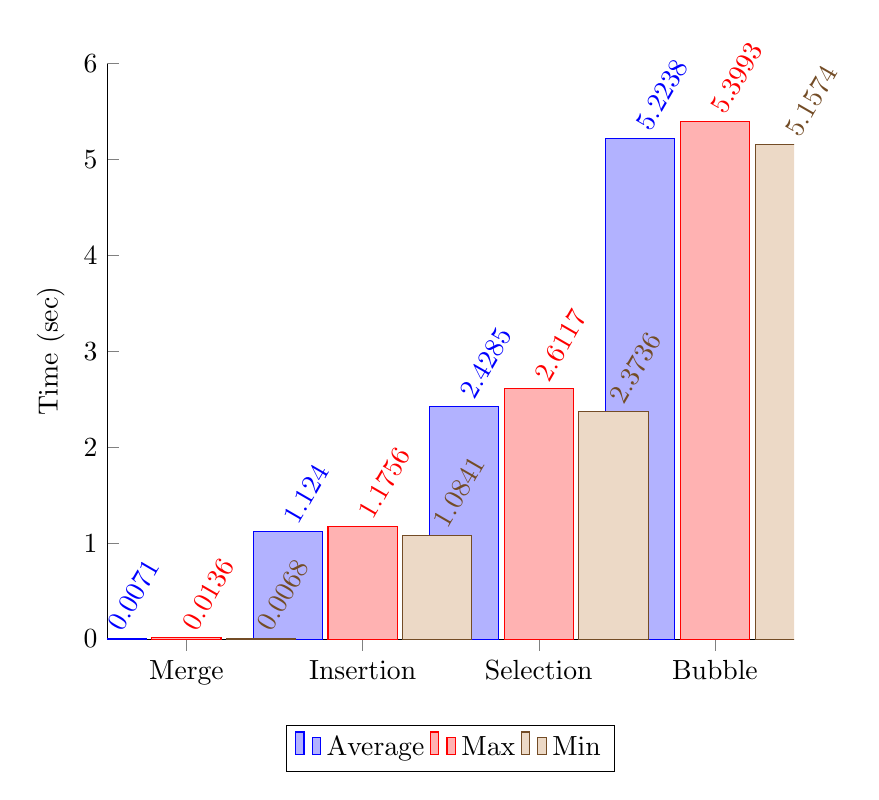
\begin{tikzpicture}
	\begin{axis}[ybar,ymin=0,ymax=6,legend style={at={(0.5,-0.15)},anchor=north,legend columns=-1},ylabel={Time (sec)},
	symbolic x coords={Merge,Insertion,Selection,Bubble},width=0.85\textwidth,bar width=25pt,
	xtick=data,axis lines*=left,enlarge x limits=0.15,
	nodes near coords={\pgfmathprintnumber[fixed, precision=4]{\pgfplotspointmeta}},
	every node near coord/.append style={anchor=mid west,rotate=60}]
	\addplot coordinates {(Merge,0.0071) (Insertion,1.1240) (Selection,2.4285) (Bubble,5.2238)};
	\addplot coordinates {(Merge,0.0136) (Insertion,1.1756) (Selection,2.6117) (Bubble,5.3993)};
	\addplot coordinates {(Merge,0.0068) (Insertion,1.0841) (Selection,2.3736) (Bubble,5.1574)};
	\legend{Average,Max,Min}
	\end{axis}
	\end{tikzpicture}\\[2mm]

	\section{Analysis}
	As can be clearly seen from the results, our sorting algorithms performed exactly as we had expected them to, with the quadratic bubble sort algorithm having the worst performance, taking an average of six seconds to sort; and the logarithmic merge sort algorithm having the best performance, taking seven milliseconds on average. My conclusion, therefore, is that the merge sort algorithm substantially outperforms any quadratic sorting algorithm in the average case, and is sufficient for processing large amounts of data.\newpage
	\section{Source Code Listing}
	\begin{lstlisting}[caption=Main.java]		
		import java.io.File;
		import java.io.FileNotFoundException;
		import java.util.ArrayList;
		import java.util.List;
		import java.util.Scanner;
		
		public class Main {
		
			// Program entry point
			public static void main(String[] args) throws FileNotFoundException {
				System.out.printf("Type in a filename: ");

                Scanner fnsc = new Scanner(System.in);
                Scanner sc = new Scanner(new File(fnsc.nextLine()));

				List<String> init_list = new ArrayList<>();
				
				System.out.println("Reading data...");
				double stTime = System.nanoTime();
				while (sc.hasNextLine()) {
					init_list.add(sc.nextLine());
				}
				double spTime = System.nanoTime();
				System.out.printf("Data read in %f sec\n\n", ((spTime - stTime) / 1000000000));
				
				// Mergesort
				System.out.print("Mergesort times (sec):\n");
				stats(new Merge(), init_list, 50);
				
				// Insertion sort
				System.out.print("Insertion sort times (sec):\n");
				stats(new Insertion(), init_list, 50);
				
				// Selection sort
				System.out.print("Selection sort times (sec):\n");
				stats(new Selection(), init_list, 50);
				
				// Bubble sort
				System.out.print("Bubblesort times (sec):\n");
				stats(new Bubble(), init_list, 50);
			}
			
			@SuppressWarnings("unchecked")
			private static <T extends Comparable<? super T>> void stats(Sort method, List<T> l, int iterations) {
				List<Double> times = new ArrayList<>();
				T[] dataset;
				
				for (int i=0;i<iterations;i++) {
					dataset = l.toArray((T[]) new Comparable[l.size()]);
					times.add(method.sort(dataset));
				}
				
				times.forEach(System.out::println);
				System.out.printf("Average: %f\n", times.parallelStream()
						.mapToDouble(t -> t)
						.average()
						.getAsDouble());
				System.out.printf("Min: %f\n", times.parallelStream()
						.mapToDouble(t -> t)
						.min()
						.getAsDouble());
				System.out.printf("Max: %f\n", times.parallelStream()
						.mapToDouble(t -> t)
						.max()
						.getAsDouble());
				System.out.printf("Total: %f\n\n", times.parallelStream()
						.mapToDouble(t -> t)
						.sum());
				times.clear();
			}
		}
	\end{lstlisting}
	\vspace{2cm}
	\begin{lstlisting}[caption=Sort.java]
		abstract class Sort {
			protected double stTime; // Start
			protected double spTime; // Stop
			
			// Returns the time it took to sort the array
			public abstract double sort(Comparable[] a);
		}
		
		@SuppressWarnings("unchecked")
		class Merge extends Sort {
			public double sort(Comparable[] a) {
				Comparable[] tmp = new Comparable[a.length];
				stTime = System.nanoTime();
				
				mergeSort(a, tmp,  0,  a.length - 1);
				
				spTime = System.nanoTime();
				return (spTime - stTime) / 1000000000;
			}
			
			private static void mergeSort(Comparable[] a, Comparable[] tmp, int left, int right) {
				if( left < right ) {
					int center = (left + right) / 2;
					mergeSort(a, tmp, left, center);
					mergeSort(a, tmp, center + 1, right);
					merge(a, tmp, left, center + 1, right);
				}
			}
			
			private static void merge(Comparable[] a, Comparable[] tmp, int left, int right, int rightEnd) {
				int leftEnd = right - 1;
				int k = left;
				int num = rightEnd - left + 1;
				
				while(left <= leftEnd && right <= rightEnd)
					if(a[left].compareTo(a[right]) <= 0)
						tmp[k++] = a[left++];
					else
						tmp[k++] = a[right++];
				
				while(left <= leftEnd)    // Copy rest of first half
					tmp[k++] = a[left++];
				
				while(right <= rightEnd)  // Copy rest of right half
					tmp[k++] = a[right++];
				
				// Copy tmp back
				for(int i = 0; i < num; i++, rightEnd--)
					a[rightEnd] = tmp[rightEnd];
			}
		}
		
		@SuppressWarnings("unchecked")
		class Insertion extends Sort {
			public double sort(Comparable[] a) {
				stTime = System.nanoTime();
				
				for (int i = 1; i < a.length; i++) {
					Comparable t = a[i];
					int j;
					for (j = i - 1; j >= 0 && t.compareTo(a[j]) < 0; j--)
						a[j+1] = a[j];
					a[j+1] = t;
				}
				
				spTime = System.nanoTime();
				return (spTime - stTime) / 1000000000;
			}
		}
		
		@SuppressWarnings("unchecked")
		class Bubble extends Sort {
			public double sort(Comparable[] a) {
				int right_border = a.length - 1;
				stTime = System.nanoTime();
				
				do {
					int last_exchange = 0;
					for (int i = 0; i < right_border; i++) {
						if (a[i].compareTo(a[i + 1]) > 0)  {
							Comparable temp = a[i];
							a[i] = a[i + 1];
							a[i + 1] = temp;
							last_exchange = i;
						}
					}
					right_border = last_exchange;
				} while ( right_border > 0 );
				
				spTime = System.nanoTime();
				return (spTime - stTime) / 1000000000;
			}
		}
		
		@SuppressWarnings("unchecked")
		class Selection extends Sort {
			public double sort(Comparable[] a) {
				int min;
				Comparable temp;
				stTime = System.nanoTime();
				
				for (int i=0; i<a.length-1; i++) {
					min = i; //index of object with minimum value
					
					for (int scan = i+1; scan < a.length; scan++)
						if (a[scan].compareTo(a[min]) < 0)
							min = scan;
					
					//swap value
					temp = a[min];
					a[min] = a[i];
					a[i] = temp;
				}
				
				spTime = System.nanoTime();
				return (spTime - stTime) / 1000000000;
			}
		}
	\end{lstlisting}
\end{document}
